\chapter{二试专题}

\newpage
\subsection*{二试练习1}

\textbf{1.}~~\textit{(szm代数原创1)}~设映射$f:\{1,\cdots ,100\} \to \{0,\cdots ,99\}$, 满足对任意$1 \leq n \leq 100$均有$f(n)<n$, 且$\sum_{n=1}^{100}f(n)=2525$. 求最小的正整数$m$, 使得必有$f^m(100)=0$. 
\vspace{24em}

\textbf{2.}~~\textit{(szm几何原创1)}~如图, 在$\triangle ABC$中, $H$是垂心, $O$是外心. $AH$交$BC$于$D$, 过$A$作$BC$的平行线, 与过$O$且垂直于$BC$的直线交于点$E$. 延长$ED$交$\odot (BOC)$于点$F$, 过$F$作直线交$\odot O$于点$G,I$. 设$AG,AI$分别交$BC$于点$J,K$, 求证: $A,H,J,K$四点共圆. 

\vspace{2em}
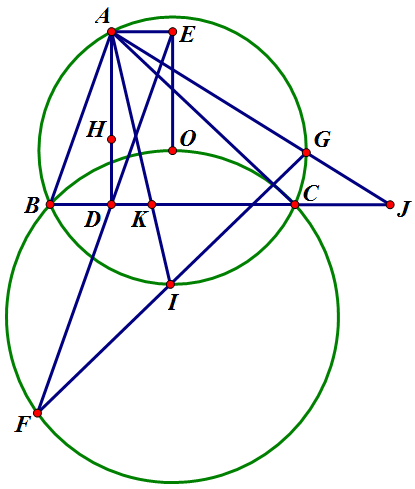
\includegraphics[width=6cm]{attachment/g1.png}


\newpage

\textbf{3.}~~\textit{(szm数论原创6)}~设数列$\{ a_n \}$满足: (1) $a_1$是完全平方数; (2) 对任意正整数$n$, $a_{n+1}$是使$$2^na_1+2^{n-1}a_2+\cdots +2a_n+a_{n+1}$$
为完全平方数的最小正整数. 若存在正整数$s$, 使得$a_s=a_{s+1}=t$, 求$t$的最小可能值. 

\vspace{22em}

\textbf{4.}~~\textit{(szm组合原创7)}~设$n,k$是给定的正整数. 在一个$n \times n$的方格表中, 甲要从左下角格走到右上角格, 每次走入有公共边的格. 乙要将$k$个格挖坑, 可以是左下角格和右上角格. 问: 乙最多能保证甲踩几个坑? 

\newpage
\subsection*{二试练习2}

\textbf{1.}~~\textit{(szm代数原创3)}~求最大的实数$C$, 使得对任意和不超过$\sqrt{2}$的非负实数$a_1,\cdots ,a_{2022}$, 均有$$\frac{1}{1+a_1^2} + \cdot + \frac{1}{1+a_{2022}^2} \geq \frac{1}{1+(a_1+\cdots +a_{2022})^2}+C.$$
\vspace{22em}

\textbf{2.}~~\textit{(szm几何原创6)}~如图, $\triangle ABC$的垂心是$H$, 外接圆是$\Omega$. $N,K$分别是边$BC$和$\Omega$上的点, 满足$NK=NH$且$A,H,K$不共线. 设$\odot (HNK)$与$\odot (ABC)$交于另一点$E$, 求证: $AE \bot NE$. 

\vspace{2em}
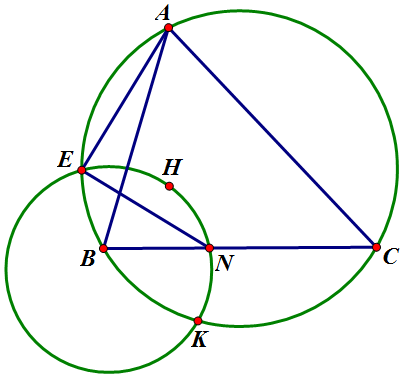
\includegraphics[width=6cm]{attachment/g6.png}

\newpage

\textbf{3.}~~\textit{(szm数论原创9)}~求证: 对任意整数$C$和正整数$n$, 存在正整数$x,y,z$, 满足$n \mid x^2+y^3+z^5+C$. 

\vspace{26em}

\textbf{4.}~~\textit{(szm组合原创7)}~设整数$n \geq 2$. 平面上有$2n$条直线, 任两条不平行, 任三条不交于一点, 此时每条直线被截为$2n$段. 对于其中的每条直线, 甲可去掉其两两不相邻的$n$段(即第$1,3,\cdots ,2n-1$段或第$2,4,\cdots ,2n$段), 剩下的部分将平面分成若干连通区域. 求连通区域个数的最小值. 

\newpage
\subsection*{二试练习3}

\textbf{1.}~~\textit{(szm几何原创4)}~如图, 在$\triangle ABC$中, $AB>AC$, $I$是内心, $M$是弧$BAC$的中点. 延长$MI$交$BC$于点$D$, 交$\odot (ABC)$于点$E$. 设$\odot (BMD)$交$BE$于$F$, 延长$DF$交$\odot (ABC)$于点$G$. 求证: $EG=EI$. 

\vspace{2em}
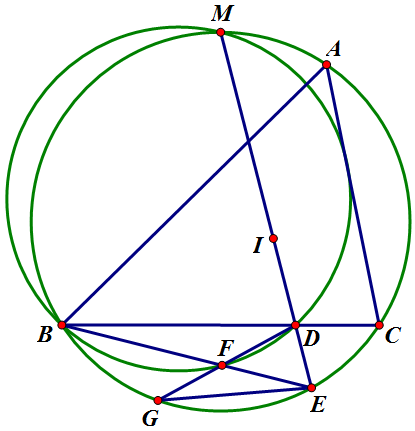
\includegraphics[width=6cm]{attachment/g4.png}

\vspace{7em}

\textbf{2.}~~\textit{(szm数论原创2)}~设$p$是奇素数. 求证: 存在无穷多个素数$q$, 使得对任意正整数$x$, $q \nmid 2^x+x^2$且$q \nmid p^x+x^2$. 

\newpage

\textbf{3.}~~\textit{(szm代数原创4)}~给定正实数$k$和正整数$n$. 对正实数$a,b,c$, 令$$f(a,b,c) = \min \left\{ \frac{k}{a}+b,\frac{k}{b}+c,\frac{k}{c}+a \right\}.$$
设正实数$a_1,\cdots ,a_n$满足$a_1+\cdots +a_n=1$, 求$\sum_{i=1}^{n}f(a_i,a_{i+1},a_{i+2})$的最小值, 其中下标按模$n$理解. 

\vspace{24em}

\textbf{4.}~~\textit{(szm组合原创15)}~有$2022$个容量均为正整数(不一定相同)的水杯排成一圈, 顺时针编号为$1,\cdots ,2022$. 一开始$1$号水杯装满水, 其余水杯均为空杯. 一次操作定义为依次对$i=1,\cdots ,2022$, 把$i$号水杯里的水尽可能多地倒入$i+1$号水杯, 使得不发生溢出(有可能前一杯倒空后下一杯还不满), 这里编号是在模$2022$意义下的. 求证: 有限次操作后将得到一个状态, 这个状态在操作下是不变的. 


\newpage
\subsection*{二试练习4}

\textbf{1.}~~\textit{(szm代数原创5)}~给定正整数$n$. 求最小的正整数$k$, 使得对任意和为$n$的正实数$a_1,\cdots ,a_n$, 均有$$n+\frac{k}{a_1 \cdots a_n} \geq k + \sum_{i=1}^{n} a_i^2.$$

\vspace{22em}

\textbf{2.}~~\textit{(szm几何原创8)}~如图, 在$\triangle ABC$中, $\angle A=60^{\circ}$, $A$-鸡爪圆交直线$AB,AC$于点$M,N$, 直线$MN$交$BC$于点$D$. 设弧$BMC$的中点为$E$, 以$ED$为直径的圆交$BC$于点$G$, 交鸡爪圆于点$F$. 求证: $A,F,G$三点共线. 

\vspace{2em}
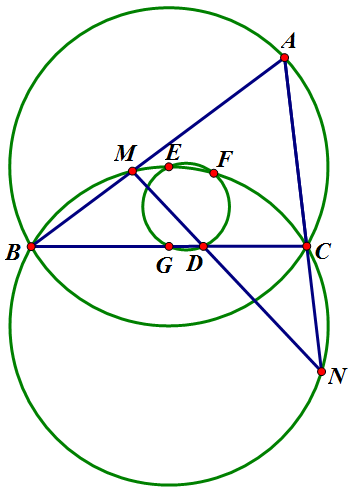
\includegraphics[width=5cm]{attachment/g8.png}


\newpage

\textbf{3.}~~\textit{(szm组合原创5)}~有$2n$张卡片, 上面写着$1 \sim n$各两张. 将它们任意排成一行, 从中拿走$1 \sim n$各一张, 剩余的卡片从左到右形成一个$1 \sim n$的排列. 对不同的初始排列方式, 求所形成的排列个数的最大值. 

\vspace{25em}

\textbf{4.}~~\textit{(szm数论原创10)}~设整数$k \geq 2$, 素数$p,q$满足$p=kq+1$. 求证: 存在正整数$m$, 使得$S(mp) \leq k+1$. 这里$S(n)$表示正整数$n$在十进制中的数码和. 


\newpage
\subsection*{二试练习5}

\textbf{1.}~~\textit{(szm代数原创6)}~设正实数$x_1,\cdots ,x_n$满足$x_1^2+\cdots +x_n^2=1$. 求证: $$\sum_{i=1}^{n} \frac{n}{1-x_i^n} \geq \frac{(1+n)^{1+1/n}}{n}.$$

\vspace{22em}

\textbf{2.}~~\textit{(szm几何原创13)}~如图, $\triangle ABC$的垂心为$H$, $BE, CF$是高, $K,M$分别是$AH,BC$的中点. 求证: $\odot (AHM), \odot (BCK)$的根轴平分线段$EF$. 

\vspace{2em}
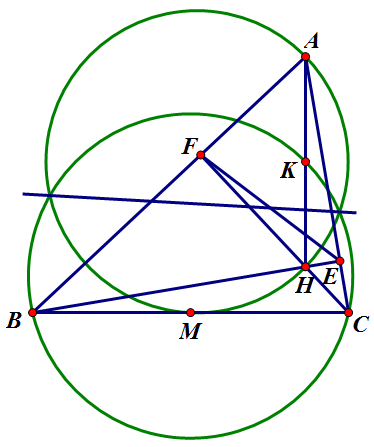
\includegraphics[width=5.5cm]{attachment/g13.png}

\newpage

\textbf{3.}~~\textit{(szm组合原创20)}~平面上任给$n$条两两无公共点的线段. 每次操作可在两条不同的线段上各取一点并连线段, 然后擦掉所有与之相交的线段(包括两点所在的两条线段). 问: 至少操作多少次能保证变为一条线段? 

\vspace{24em}

\textbf{4.}~~\textit{(szm数论原创12)}~用$\omega (n)$表示正整数$n$的不同素因子的个数, 其中$\omega (1)=0$. 求证: 对任意正整数$a,b$, $$\sum_{i=a+1}^{a+b} 2^{\omega (i)} > \sum_{i=1}^{b} 2^{\omega (i)}.$$




\newpage
\subsection*{二试练习6}

\textbf{1.}~~\textit{(szm数论原创8)}~对正整数$m<n$, 若存在正整数$m',n'$, 满足$m<m' \leq n' <n$, 且$mn=m'n'$, 则称$(m,n)$为\textit{可缩的}. 求证: 对任意正整数$t$, 存在正整数$a_1<\cdots <a_t$, 使得$(a_1,a_2),\cdots ,(a_{t-1},a_t)$可缩, 而$(a_1,a_t)$不可缩. 

\vspace{24em}

\textbf{2.}~~\textit{(szm代数原创8)}~给定正实数$n$. 设和为$1$的正实数$a_1,\cdots ,a_n$. 对$1 \leq i \leq n$, 用$f(i)$表示$a_1,\cdots ,a_i$中小于等于$a_i$的个数. 求最大的实数$c$, 使得总有$\sum_{i=1}^{n} a_{f(i)} \geq c$. 

\newpage

\textbf{3.}~~\textit{(szm几何原创15)}~如图, $\odot O$和$\odot I$分别是$\triangle ABC$的外接圆和内切圆, $P$是两圆的外位似中心, 延长$AP$交$\odot I$于点$G$. 过$B,C$作$AI$的垂线, 垂足分别为$D,E$, 设以$DE$为直径的圆与$\odot I$的根轴为$\ell$. 求证: $\ell$, $BC$, $\odot I$在$G$处的切线交于一点$K$. 

\vspace{2em}
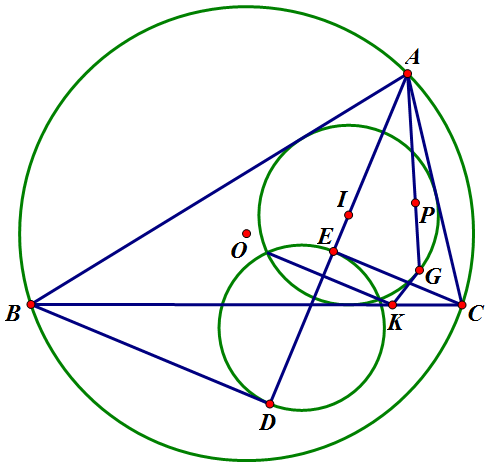
\includegraphics[width=7cm]{attachment/g15.png}

\vspace{8em}

\textbf{4.}~~\textit{(szm组合原创22简化)}~Jerry和一些Tom在一个圆形花园(即圆的内部或边界)里玩抓人游戏. 若某一时刻至少一个Tom与Jerry在同一位置, 则认为Jerry被抓到. 已知Tom和Jerry的移动速度相同, 且它们互相都能看到对方的位置. 问: 至少需要几个Tom才能抓到Jerry? 


\newpage
\subsection*{二试练习6}

\textbf{1.}~~\textit{(szm数论原创13)}~对正整数$n$, 记$$\sigma _n := \prod_{p\text{~prime}} p^{\lfloor \frac{n}{p-1} \rfloor}.$$
求证: $(n+1)! \mid \sigma _n$且$\sigma _n \mid n! [1,\cdots ,n+1]$. 

\vspace{20em}

\textbf{2.}~~\textit{(szm几何原创16)}~如图, 在$\triangle ABC$中, $AD$是高, $F,E,M$分别是$AB,AC,BC$上的点, 满足$E,A,F,M,D$五点共圆. 延长$DF,DE$, 分别交$\odot (BDE), \odot (CDF)$于点$H,G$. $K,L$分别是$\odot (BDE), \odot (CDF)$上的点, 满足$\angle HKF =\angle GLE = 90^{\circ}$. 求证: $K,L,M,D$四点共圆. 

\vspace{2em}
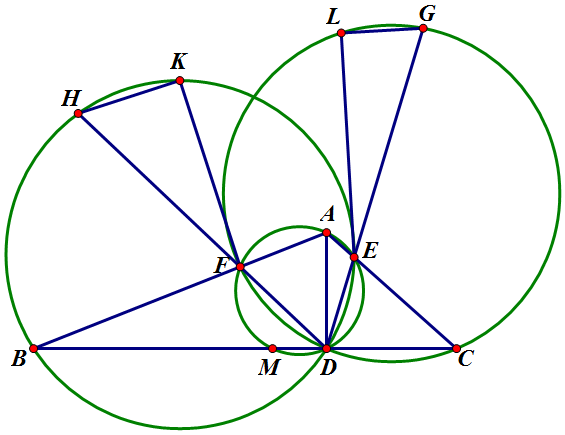
\includegraphics[width=7.5cm]{attachment/g16.png}

\newpage

\textbf{3.}~~\textit{(szm组合原创14)}~设数列$\{ a_n \}$满足, 对任意正整数$i$, 可重集$A_i=\{ a_1,\cdots ,a_i \}$可从可重集$B_i=\{ a_{i+1},\cdots ,a_{2i+1} \}$中去掉一个元素得到. 对给定的正整数$k$, 求最小的正整数$n_k$, 使得$a_1 \sim a_{n_k}$中可能有$k$个不同的值. 

\vspace{24em}

\textbf{4.}~~\textit{(szm代数原创11)}~设$y_1,\cdots ,y_n$和$\frac{x_1}{y_1},\cdots ,\frac{x_n}{y_n}$均为不减的正数数列, 满足$\sum_{i=1}^{n}x_i = \sum_{i=1}^{n} y_i$. 求证: $$\sum_{\varnothing \neq S \subseteq \{ 1,\cdots ,n \}} \frac{\sum_{i \in S}x_i}{\sum_{i \in S}y_i} \leq 2^n-1.$$








\newpage
\subsection*{二试练习7}

\textbf{1.}~~\textit{(szm数论原创21)}~设$p$是奇素数, $a$是大于$1$的整数. 定义多项式$$f_k(x) = \prod_{j=1}^{a-1} (xp^j-k),\qquad g(x) = x\prod_{k=1}^{p-1} f_k(x).$$
求证: $g(1),\cdots ,g(p^a)$构成模$p^a$的一个完全剩余系. 

\vspace{21em}

\textbf{2.}~~\textit{(szm几何原创17)}~如图, $H$是$\triangle ABC$的垂心, $A'$是$A$的对径点. $D$是$BC$上一点, $E$是$D$在$AB$上的投影, $B'$是$AB$上的点, 使得$B'E=BE$. 延长$A'D$交$\odot (ABC)$于点$P$, 延长$BC$与$\odot (BB'P)$于点$X$. 求证: $\angle HXC = \angle EPB'$. 

\vspace{2em}
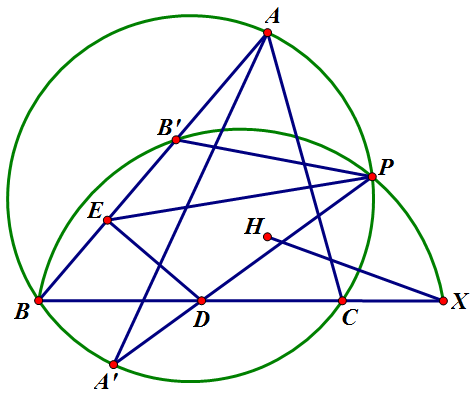
\includegraphics[width=7cm]{attachment/g17.png}

\newpage

\textbf{3.}~~\textit{(szm代数原创13)}~设$n$是正整数, $a_1,\cdots a_{n^2}$为正实数, 满足$a_1^2 + \cdots +a_{n^2}^2 =1$. 求证: $$(n-1)^{n^2}a_1\cdots a_{n^2} \leq (1-a_1)\cdots (1-a_{n^2}).$$

\vspace{23em}

\textbf{4.}~~\textit{(szm组合原创23)}~一个形如半径为$1$的圆的“欢乐动物园”的圆心有一只“欢乐马”, 在其边界上有$t$个管理员. 欢乐马可在平面上自由移动, 而管理员仅可在他们的初始位置的凸包的边界上移动, 并且所有人和动物的速度均不超过$1$. 当欢乐马与管理员的位置重合时, 则视为管理员抓住欢乐马. 当欢乐马达到圆外时, 则视为它逃离欢乐动物园. 求$t$的最大值, 使得欢乐马可以在不被管理员抓住的情况下, 逃离欢乐动物园. 




\newpage
\subsection*{二试练习8}

\textbf{1.}~~\textit{(szm代数原创14)}~设$x_1,\cdots ,x_{2022}$是和为$1$的非负实数, 满足$\sum_{i=1}^{2022}x_ix_{i+1}=\frac{1}{2000}$, 其中$x_{2023}=x_1$. 求证: 存在$i,j \in \{ 1,\cdots ,2022 \}$, 使得$|x_i-x_j|>10^{-5}$. 

\vspace{24em}

\textbf{2.}~~\textit{(szm几何原创18)}~如图, 在$\triangle ABC$中, $AB < AC$, $\odot O$是外接圆. $\odot O$在$A$处的切线与直线$BC$交于点$P$, $D$是$PO$上的一点使得$BD=OD$. 延长$BD$交$\odot O$于点$F$, 过$F$作$AC$的平行线交$\odot O$于点$G$, 过$A$作$AB$的垂线交$BF$于点$E$, 延长$CE$交$AG$于点$H$. 求证: $DH \bot AC$. 


\vspace{2em}
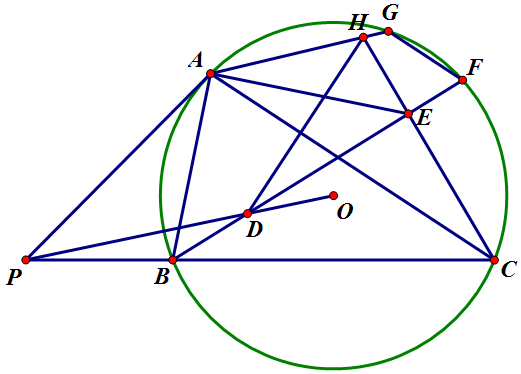
\includegraphics[width=7cm]{attachment/g18.png}

\newpage

\textbf{3.}~~\textit{(szm数论原创19)}~设$K$和$a_1 <\cdots <a_{n+1}$是正整数. 若对任意$1 \leq i \leq n$, 都有$K \equiv a_i \mod a_{i+1}$, 求证: $K>\frac{n^2}{4}$. 

\vspace{24em}

\textbf{4.}~~\textit{(szm组合原创24)}~$K$岛是一个面积为$520$的没有湖泊的小岛, 它的海岸线是一个简单$1000$边形. 小林在岛上的某处种下一朵盛开的蒲公英, 它的无数种子向四面八方沿直线传播, 并有可能在任何时刻落在地面上, 但所有种子至多只能飞越一道海湾. 不久后, 岛上所有种子萌发. 试问小林是否一定能保证此时岛上有面积不小于$\pi$的蒲公英花海? 

\newpage
\subsection*{二试练习9}

\textbf{1.}~~\textit{(szm代数原创22)}~给定正整数$n$. 设正实数$a_1,\cdots ,a_n$满足$\sum_{k=1}^{n}a_k=n$. 求最大的实数$\lambda$, 使得恒有$$\sum_{k=1}^{n} a_k^2 \leq n\left( n-\lambda\left( \prod_{k=1}^{n}a_k \right)^{1/n} \right)^2.$$

\vspace{22em}

\textbf{2.}~~\textit{(szm几何原创19)}~如图, 在$\triangle ABC$中, $AB>AC$, $M$是弧$BAC$的中点. 延长$MA,BC$交于点$D$. 过$D$且与$BC$相切的圆$\Gamma$交$\odot (ABC)$于弧$BC$上的两点$E,F$, 延长$MF$交$\Gamma$于点$T$. $G$是$\Gamma$上一点, 满足$\angle BGC = \angle CAD$, 过$G$作$ET$的垂线交$BD$于点$X$. 求证: 若$\angle EAB + \angle CAD = 90^{\circ}$, 则$XG$与$\odot (ABC)$相切. 

\vspace{2em}
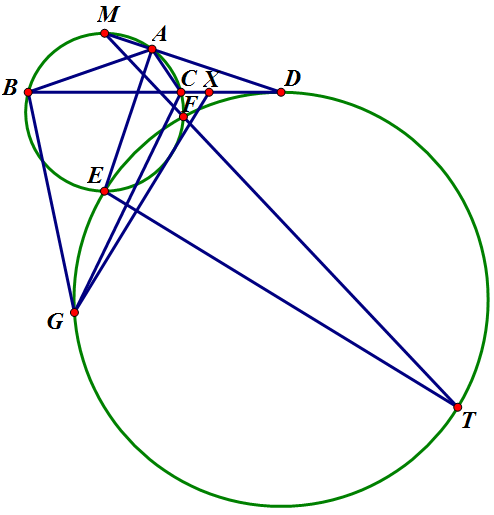
\includegraphics[width=7cm]{attachment/g19.png}

\newpage

\textbf{3.}~~\textit{(szm数论原创29)}~求所有的正整数$n$, 满足$$\lfloor \sqrt{2}n \rfloor ^2 + 4\lfloor \sqrt{2}n \rfloor = 2n^2+4n.$$

\vspace{24em}

\textbf{4.}~~\textit{(szm组合原创25)}~设$a_1,\cdots ,a_n$是$1,\cdots ,n$的一个排列. 对$1 \leq i \leq n$, 设以$a_i$为首项的最长递增子列的长度为$x_i$, 最长递减子列的长度为$y_i$. 求正整数$k$的最大可能值, 使得存在$k$个正整数$1 \leq i_1 < \cdots <i_k \leq n$, 满足$x_{i_1} > \cdots >x_{i_k}$且$y_{i_1} > \cdots >y_{i_k}$. 

\newpage
\subsection*{二试练习10}

\textbf{1.}~~\textit{(szm代数原创23)}~给定正整数$n \geq 2$. 求最小的实数$\lambda$, 使得对任意和为$1$的正实数$a_1,\cdots ,a_n$, 都有$$\sum_{k=1}^{n} \frac{a_k^2+\lambda a_{k+1}}{\sum_{j \neq k}a_j} \geq \frac{n+1}{n-1}.$$

\vspace{21em}



\textbf{2.}~~\textit{(szm几何原创20)}~如图, $\triangle ABC$的外心和垂心分别为$O,H$. 设$AH$与$BC$交于点$H_1$, 以$AH$为直径的圆与$\odot O$的另一个交点为$P$, 延长$PH_1$交$\odot O$于点$T$. 过$H$作$OH_1$的平行线与弧$BAC$交于点$Q$. 求证: $QT$过$BC$中点$M$. 

\vspace{2em}
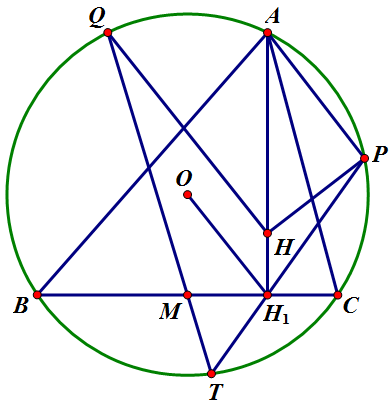
\includegraphics[width=6cm]{attachment/g20.png}


\newpage

\textbf{3.}~~\textit{(szm数论原创36)}~求所有的正整数$t$, 使得对无穷个正整数$n$, 存在正整数$a_{ij}(1 \leq i,j \leq n)$, 满足$$(a_{11},\cdots ,a_{1n}),\cdots ,(a_{t1},\cdots ,a_{tn}),(a_{11} \cdots a_{t1} ,\cdots ,a_{1n} \cdots a_{tn})$$
均为模$n$的完全剩余系. 

\vspace{23em}

\textbf{4.}~~\textit{(szm组合原创37)}~给定整数$x \geq 2$. MO星球的“世界杯”小组赛如下进行: 每个小组有$2x$个国家的球队, 采用单循环赛制, 每支球队赢一场积$3$分, 平一场积$1$分, 输一场积$0$分. 最终总积分排名前$x$位的球队晋级, 其余球队淘汰, 如果有平分出现, 则根据净胜球等其他指标决出优胜者. 设此规则下淘汰球队的最高可能积分为$M(x)$, 晋级球队的最低可能积分为$m(x)$. 求$M(x)$和$m(x)$. 


\newpage

\subsection*{数学竞赛唐题(欣赏题)集}

\textbf{1.}~~设$ABCDEF$为非凸的, 不自交的六边形, 对边都不平行. 其内角满足$\angle A = 3\angle D, \angle E = 3\angle B, \angle C = 3\angle F$. 求证: 若$|AB|=|DE|,|BC|=|EF|,|CD|=|FA|$, 则$AD,BE,CF$三线共点. 

\newpage
\textbf{2.}~~设$A$是一个$225$元集合, $A_1,\cdots ,A_{11}$是$A$的$11$个$45$元子集, 满足对任意$1\leq i<j \leq 11, |A_i \cap A_j|=9$. 求证: $|A_1 \cup \cdots \cup A_{11}| \geq 165$. 

\newpage
\textbf{3.}~~设整数$n \geq 2$. 实数$x_1,\cdots ,x_n$满足$$x_1+\cdots +x_n=0,\qquad x_1^2+\cdots +x_n^2=1.$$
对于$\{ 1,\cdots ,n \}$的子集$A$, 定义$\displaystyle S_A= \sum_{i \in A}x_i$. 求证: 对于任意正数$\lambda$, 满足$S_A \geq \lambda$的集合$A$的个数不超过$\dfrac{2^{n-3}}{\lambda ^2}$, 并给出取等情况. 














